\documentclass[tikz]{standalone}
\usepackage{pgfplots}
\pgfplotsset{compat=1.15}
\usepackage{mathrsfs}
\usetikzlibrary{arrows,calc}
\usepackage{tkz-euclide}
\pagestyle{empty}

\definecolor{AngleClr}{rgb}{0,0.39215686274509803,0}
\definecolor{ShapeClr}{rgb}{0.6,0.2,0}
\definecolor{SquareClr}{RGB}{250, 248, 217}

\begin{document}

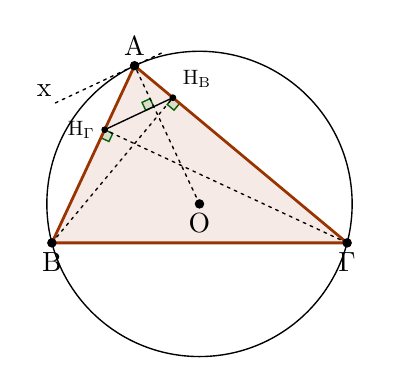
\begin{tikzpicture}[scale=.75]
\tkzSetUpLine[line width=1pt,color=black]
\tkzSetUpPoint[fill=black]

\tkzDefPoints{0/0/B,1.4/3/A,5/0/C}


\tkzDefPointBy[projection=onto B--C](A)\tkzGetPoint{HA}
\tkzDefPointBy[projection=onto A--C](B)\tkzGetPoint{HB}
\tkzDefPointBy[projection=onto A--B](C)\tkzGetPoint{HC}


\tkzDefTriangleCenter[circum](A,B,C) \tkzGetPoint{O}

\tkzDefLine[tangent at=A](O) \tkzGetPoint{x}

\tkzInterLL(HB,HC)(O,A) \tkzGetPoint{KA}
\tkzInterLL(HA,HB)(O,C) \tkzGetPoint{KC}
\tkzInterLL(HC,HA)(O,B) \tkzGetPoint{KB}

\tkzFillPolygon[fill=ShapeClr,fill opacity=0.1](A,B,C)
\tkzMarkRightAngles[line width=0.5pt, size=.15,color=AngleClr,fill=AngleClr,fill opacity=0.1](A,KA,HC B,HC,C C,HB,B)

\tkzDrawPolygon[color=ShapeClr](A,B,C)

\tkzDrawPoints[size=3](A,B,C,O)
\tkzDrawPoints[size=2](HB,HC)

\tkzDrawSegments[line width=0.5pt,color=black,dashed,dash pattern=on 1pt off 1.75pt](B,HB C,HC O,A)
\tkzDrawSegments[line width=0.5pt,color=black](HB,HC)
\tkzDrawSegments[line width=0.5pt,color=black,dashed,dash pattern=on 1pt off 1.75pt,add=0.5 and 0.5](A,x)

\tkzDrawCircle[line width=0.5pt,color=black](O,A)

\tkzLabelPoint[above](A){$\rm A$}
\tkzLabelPoint[below](B){$\rm B$}
\tkzLabelPoint[below](C){$\rm \Gamma$}
\tkzLabelPoint[below](O){$\rm O$}
\tkzLabelPoint[above right](HB){\scalebox{0.75}{$\rm H_B$}}
\tkzLabelPoint[left](HC){\scalebox{0.75}{$\rm H_\Gamma$}}
\tkzLabelPoint[left=0.25cm](x){$\rm x$}

\end{tikzpicture}

\end{document}
